% Bilag til synopsen "Fælles aner" — kodeeksempler, figurer og udviklingsproces.
% Kompileres med: pdflatex bilag.tex   (MiKTeX, dansk tegnsæt via inputenc/T1)
% Kodeuddragene er hentet fra src/ på dev-branchen (okt. 2026; docstrings er
% udeladt eller forkortet); figurene
% genereres af synopsis/figurer/make_figures.py.
\documentclass[12pt, a4paper]{article}
\usepackage[utf8]{inputenc}
\usepackage[T1]{fontenc}
\usepackage{lmodern}
\usepackage{geometry}
\geometry{margin=2.5cm}
\usepackage{amsmath, amssymb}
\usepackage{graphicx}
\usepackage{booktabs}
\usepackage{listings}
\usepackage{xcolor}
\usepackage{caption}
\usepackage[colorlinks=true, linkcolor=blue, urlcolor=blue]{hyperref}

\lstset{
    basicstyle=\ttfamily\small,
    keywordstyle=\color{blue},
    commentstyle=\color{gray},
    stringstyle=\color{teal},
    numbers=left,
    numberstyle=\tiny\color{gray},
    breaklines=true,
    frame=single,
    tabsize=4,
    showstringspaces=false,
    literate={æ}{{\ae}}1 {ø}{{\o}}1 {å}{{\aa}}1
             {Æ}{{\AE}}1 {Ø}{{\O}}1 {Å}{{\AA}}1
             {§}{{\S}}1 {—}{{---}}1 {–}{{--}}1
             {Θ}{{$\Theta$}}1 {α}{{$\alpha$}}1 {φ}{{$\varphi$}}1
             {≤}{{$\leq$}}1 {→}{{$\rightarrow$}}1 {∪}{{$\cup$}}1
             {Ē}{{$\bar{E}$}}1 {⁻}{{$^-$}}1 {̃}{{\~{}}}1
}

\title{Bilag til synopse --- \textit{Fælles aner}}
\author{[projektdeltagere]}
\date{}

\begin{document}
\maketitle

% ═════════════════════════════════════════════════════════════════════════════
\section*{Bilag A. Programstruktur og MVC-arkitektur}
% ═════════════════════════════════════════════════════════════════════════════

Projektet er opdelt i de tre MVC-lag, som opgaven kræver (Projekt.docx). Lagene
kommunikerer i én retning: modellen beregner, controlleren orkestrerer, og
views får færdige værdier og præsenterer dem.

\begin{center}
\begin{tabular}{@{}llp{6,6cm}@{}}
\toprule
\textbf{Lag} & \textbf{Moduler} & \textbf{Rolle} \\
\midrule
Model & \texttt{person.py}, \texttt{graph\_model.py}, & Data (\texttt{Person},
\texttt{FamilyGraph}) og algoritmer \\
      & \texttt{cluster\_map.py}, \texttt{search.py} & (klusterkort, rekursiv søgning) \\
View & \texttt{draw.py}, \texttt{view.py} & Lagdelt Sugiyama-layout, Mermaid/Graphviz-uddrag,
matplotlib-figurer \\
Controller & \texttt{controller.py}, \texttt{\_\_main\_\_.py} & \texttt{FamilyController}-facade
+ indgangspunkt, der driver pipelinen \\
\bottomrule
\end{tabular}
\end{center}

Kørsel: \texttt{poetry run python src} (svarende til \texttt{poetry run python -m src}).
Programmet skriver desuden figurer til \texttt{out/cluster\_<id>.png}.

% ═════════════════════════════════════════════════════════════════════════════
\section*{Bilag B. Kodeeksempler}
% ═════════════════════════════════════════════════════════════════════════════

% ─────────────────────────────────────────────────────────────────────────────
\subsection*{B1. Datamodellen: klasser og OOP (\texttt{src/person.py})}
% ─────────────────────────────────────────────────────────────────────────────

\texttt{Pronouns} er en \emph{frossen} dataklasse: attributterne kan ikke ændres
efter oprettelsen (immutabilitet), og \texttt{PRESETS} er en klassevariabel, som
deles af alle instanser.

\begin{lstlisting}[language=Python]
@dataclass(frozen=True)
class Pronouns:
    subject: str
    object: str
    possessive_adjective: str
    possessive_pronoun: str
    reflexive: str

    PRESETS: ClassVar[dict[str, Pronouns]] = {}
\end{lstlisting}

\texttt{Person} er den mutable modpart: en person skal kunne tildeles forældre
under opbygningen af familiedata. Hvert objekt gemmer højst to forældreferencer
(\texttt{mom}/\texttt{dad}), hvilket er invariant \textbf{I1} fra designdokumentet:
$\deg^{-}(v) \le 2$. Specialmetoden \texttt{\_\_str\_\_} gør objektet læsbart
ved udskrift.

\begin{lstlisting}[language=Python]
class Person:
    def __init__(
        self,
        name: str = "John Doe",
        mom: Person | None = None,
        dad: Person | None = None,
        pronouns: Pronouns | None = None,
    ):
        self.mom = mom
        self.dad = dad
        self.name = name
        self.pronouns = pronouns or Pronouns.from_preset("they")

    def __str__(self) -> str:
        known: list[str] = []
        if self.mom:
            known.append(f"mother is {self.mom.name}")
        if self.dad:
            known.append(f"father is {self.dad.name}")

        if not known:
            return f"{self.name} has no known parents."
        if len(known) == 1:
            # exactly one parent known: name the *other* one as the unknown slot
            known.append("no known father" if self.mom else "no known mother")

        return f"{self.name}'s " + " and ".join(known) + "."
\end{lstlisting}

% ─────────────────────────────────────────────────────────────────────────────
\subsection*{B2. Grafrepræsentationen (\texttt{src/graph\_model.py})}
% ─────────────────────────────────────────────────────────────────────────────

\texttt{FamilyGraph} er en frossen dataklasse med tætte heltals-id'er (O4) og et
omvendt forældre-til-barn-index, som bygges \emph{en gang} (O1). Nabolaget i den
udretningsløse skygge $\bar{E}$ er forældre $\cup$ børn --- klustertilhørighed er
ligeglad med orientering.

\begin{lstlisting}[language=Python]
    def neighbours(self, p: Person) -> tuple[Person, ...]:
        # Undirected neighbourhood in E-bar (parents u children), self-loops dropped.
        seen: set[Person] = {p}
        out: list[Person] = []
        for q in (p.mom, p.dad, *self.child_index.get(p, ())):
            if q is not None and q not in seen:
                seen.add(q)
                out.append(q)
        return tuple(out)
\end{lstlisting}

% ─────────────────────────────────────────────────────────────────────────────
\subsection*{B3. Rekursiv søgning som mindste fast punkt (\texttt{src/search.py})}
% ─────────────────────────────────────────────────────────────────────────────

Klusteret omkring en start-person $v$ er det \emph{mindste faste punkt} for
operatoren
\[
    \Phi_v(S) = \{v\} \cup \bigcup_{\{u,w\}\in\bar{E},\, u\in S}\{w\}.
\]
(Knaster--Tarski). \texttt{visited}-vagten er netop fast-punkt-stabiliseringen:
hvert knudepunkt udvides præcis én gang, så $T = \Theta(n + m) = \Theta(n)$.

\begin{lstlisting}[language=Python]
def explore(
    node: Any,
    visited: set[Any],
    members: list[Any],
    neighbours: NeighboursFn | None = None,
) -> None:
    if node is None or node in visited:
        return
    visited.add(node)
    members.append(node)
    for w in _neighbours(node, neighbours):
        explore(w, visited, members, neighbours)
\end{lstlisting}

Rekursionen er den læsbare reference. Produktionsvejen (O5) er den iterative
variant, fordi en ren kæde har dybde $\Theta(n)$, mens CPython kun har
$R = 1000$ rammer:

\begin{lstlisting}[language=Python]
def explore_iterative(
    node: Any,
    members: set[Any] | None = None,
    neighbours: NeighboursFn | None = None,
) -> set[Any]:
    seen = members if members is not None else set()
    if node is None:
        return seen
    stack = [node]
    while stack:
        current = stack.pop()
        if current is None or current in seen:
            continue
        seen.add(current)
        stack.extend(w for w in _neighbours(current, neighbours) if w not in seen)
    return seen
\end{lstlisting}

% ─────────────────────────────────────────────────────────────────────────────
\subsection*{B4. Union-Find og identitet (3) (\texttt{src/cluster\_map.py})}
% ┐────────────────────────────────────────────────────────────────────────────

Union-Find med union-efter-rang og path-halving forbinder kanter i nær-konstant
amortiseret tid. Antallet af klustre følger den afkassede identitet (3)
(Theorem 3.3):
\[
    k = n - s, \qquad s = \text{antal vellykkede } \texttt{union}\text{-kald}.
\]

\begin{lstlisting}[language=Python]
class UnionFind:
    __slots__ = ("parent", "rank", "successful_unions")

    def __init__(self, n: int):
        self.parent = list(range(n))
        self.rank = [0] * n
        self.successful_unions = 0

    def find(self, x: int) -> int:
        while self.parent[x] != x:
            self.parent[x] = self.parent[self.parent[x]]  # path halving (O3)
            x = self.parent[x]
        return x

    def union(self, a: int, b: int) -> bool:
        ra, rb = self.find(a), self.find(b)
        if ra == rb:
            return False
        if self.rank[ra] < self.rank[rb]:  # union by rank: serve the shallower root
            ra, rb = rb, ra
        self.parent[rb] = ra
        if self.rank[ra] == self.rank[rb]:
            self.rank[ra] += 1
        self.successful_unions += 1
        return True
\end{lstlisting}

% ─────────────────────────────────────────────────────────────────────────────
\subsection*{B5. Memoisering af forfædre-udregningen (\texttt{src/search.py})}
% ─────────────────────────────────────────────────────────────────────────────

Uden cache er rekursionen $\mathrm{Anc}(v) = \{v\} \cup \mathrm{Anc}(\mathrm{mom}(v))
\cup \mathrm{Anc}(\mathrm{dad}(v))$ eksponentiel ved pedigree-collapse (I3):
$\Theta(\varphi^{d})$ for Fibonacci-stamtavler. Med memoisering beregnes hvert
knudepunkt præcis én gang, så $T = \Theta(n + m)$.

\begin{lstlisting}[language=Python]
def ancestors(p: Any) -> frozenset[Any]:
    cache: dict[Any, frozenset[Any]] = {}

    def closure(node: Any) -> frozenset[Any]:
        if node is None:
            return frozenset()
        hit = cache.get(node)
        if hit is not None:
            return hit
        out = {node} | set(closure(node.mom)) | set(closure(node.dad))
        cache[node] = frozenset(out)
        return cache[node]

    return closure(p)
\end{lstlisting}

Den iterative variant \texttt{ancestors\_iterative} beregner samme lukning med
eksplicit stak (O5) og rejser \texttt{CycleError} ved forældrecyklusser i stedet
for at køre fast.

% ─────────────────────────────────────────────────────────────────────────────
\subsection*{B6. Tegning af klusterkortet: Sugiyama-layout (\texttt{src/draw.py})}
% ┐────────────────────────────────────────────────────────────────────────────

Første gennemløb tildeler generationer som længste-vej-rang (Kahn's algoritme);
et barn ligger præcis én generationsskridt under begge forældre. Et cyklus-tjek
rejses \emph{før} layoutet, hvis data ikke opfylder invariant \textbf{I2}.

\begin{lstlisting}[language=Python]
    ranks = {v: 0 for v in members}
    indegree = {v: len(parents[v]) for v in members}
    ready = deque(
        sorted((v for v in members if indegree[v] == 0), key=lambda p: p.name)
    )
    processed = 0
    while ready:
        parent = ready.popleft()
        processed += 1
        for child in children[parent]:
            ranks[child] = max(
                ranks[child], ranks[parent] + delta
            )  # longest path (§6.1)
            indegree[child] -= 1
            if indegree[child] == 0:
                ready.append(child)
    if processed != len(members):
        raise CycleError("cycle in parental record — layered layout needs a DAG (I2)")
\end{lstlisting}

Andet gennemløb minimerer kanter der krydser hinanden med barycenter-heuristikken
$b(u) = \frac{1}{\deg(u)}\sum_{w \in \bar{E}(u)} \mathrm{pos}(w)$ --- problemet er
NP-hardt i almindelighed, så en heuristik er den accepterede løsning:

\begin{lstlisting}[language=Python]
        def bary(node: Any) -> tuple[float, int]:
            nbs = neighbours[node]
            if not nbs:
                return float(pos[node]), pos[node]  # isolated: keep position
            b = sum(pos[w] for w in nbs if w in pos) / len(nbs)
            return b, pos[node]

        nodes.sort(key=bary)  # stable: ties broken by current position
\end{lstlisting}

% ─────────────────────────────────────────────────────────────────────────────
\subsection*{B7. Visualisering med matplotlib.pyplot (\texttt{src/view.py})}
% ─────────────────────────────────────────────────────────────────────────────

View-laget oversætter layout-koordinaterne til en figur: én boks pr. person ved
$(x, y) = (\text{position i laget}, \text{rang})$, og en pil pr. forældreferens
fra forælder til barn --- samme orientering som Mermaid- og Graphviz-uddragene.

\begin{lstlisting}[language=Python]
    for child, parent in cluster.edges:  # (child, parent) per §1.1
        ax.annotate(
            "",
            xy=(layout.x[child] * X_GAP, layout.ranks[child]),
            xytext=(layout.x[parent] * X_GAP, layout.ranks[parent]),
            arrowprops={"arrowstyle": "->", "color": EDGE_COLOR, "lw": 1.2,
                        "shrinkA": 10, "shrinkB": 10},
        )
    for person in members:
        ax.text(
            layout.x[person] * X_GAP,
            layout.ranks[person],
            label(person),
            ha="center",
            va="center",
            fontsize=9,
            bbox=HIGHLIGHT_STYLE if person in hot else NODE_STYLE,
        )
\end{lstlisting}

% ═════════════════════════════════════════════════════════════════════════════
\section*{Bilag C. Visualisering af træet}
% ═════════════════════════════════════════════════════════════════════════════

\begin{figure}[h]
\centering
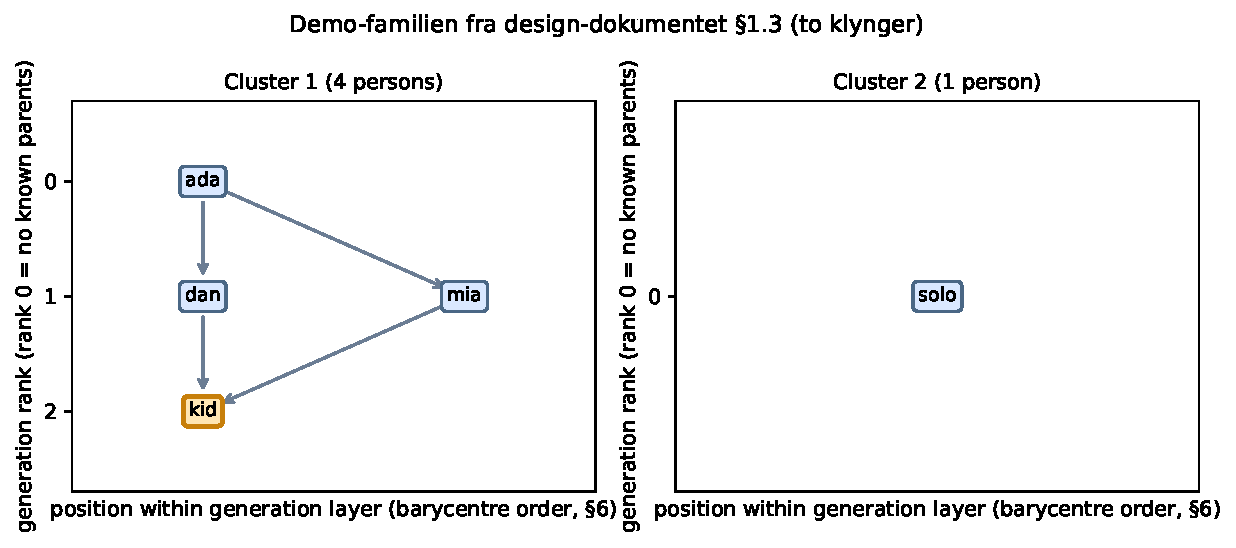
\includegraphics[width=0.95\textwidth]{figurer/familie_demo.pdf}
\caption{Demo-familien fra design-dokumentet \S 1.3 tegnet af programmets eget
view-modul. To klynger: sammenbrudsfamilien til venstre (ada er både mias og dans
far, hvilket er pedigree-collapse, invariant \textbf{I3}) og den isolerede person
\texttt{solo} til højre. Søgeudgangspunktet \texttt{kid} er fremhævet.}
\end{figure}

\begin{figure}[h]
\centering
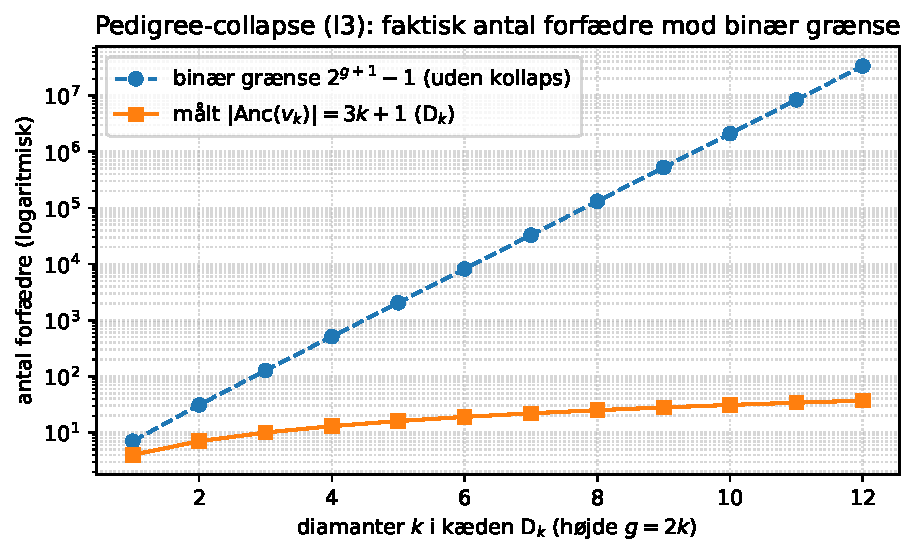
\includegraphics[width=0.8\textwidth]{figurer/pedigree_collapse.pdf}
\caption{Pedigree-collapse i tal: for diamantkæden $D_k$ er det faktiske antal
forfædre $|\mathrm{Anc}(v_k)| = 3k+1$, mens den naive bin{\ae}re gr{\ae}nse
$2^{g+1}-1$ vokser eksponentielt med h{\o}jden $g = 2k$. M{\aa}lt med programmets
\texttt{ancestors\_iterative}.}
\end{figure}

\begin{figure}[h]
\centering
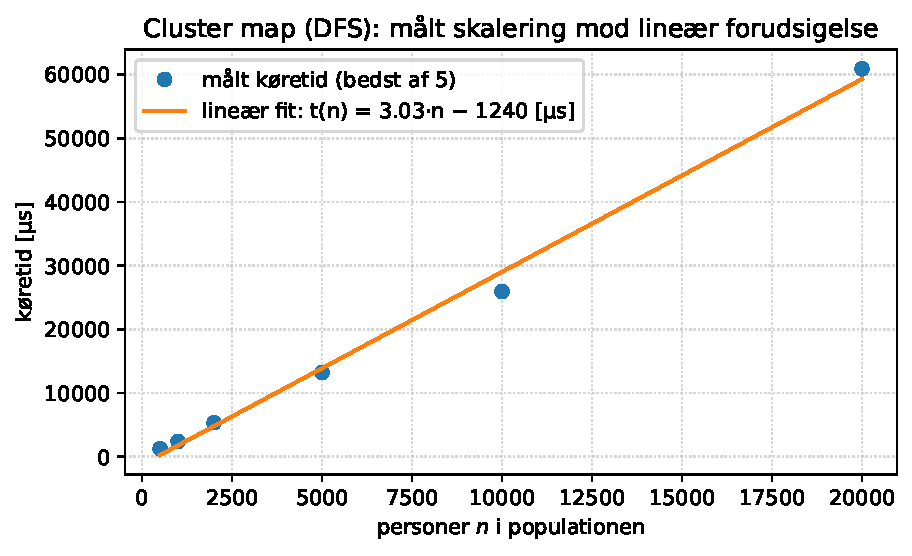
\includegraphics[width=0.8\textwidth]{figurer/scaling.pdf}
\caption{M{\aa}lt k{\o}retid for klusterkort-konstruktionen (DFS) vha.
\texttt{time.perf\_counter}, bedst af 5 gentagelser pr. punkt. Den line{\ae}re
fit $t(n) \approx c \cdot n$ bekr{\ae}fter kompleksitetsanalysen
$T = \Theta(n + m) = \Theta(n)$ fra \S 4.1 (invariant \textbf{I1} giver
$m \le 2n$).}
\end{figure}

% ═════════════════════════════════════════════════════════════════════════════
\section*{Bilag D. Udviklingsprocessen (Git)}
% ═════════════════════════════════════════════════════════════════════════════

Koden er udviklet på \texttt{dev}-branchen i repoet
\begin{center}
\url{https://github.com/ExperiencesXP/proj_herritage_tree}
\end{center}
Commit-oversigten pr. 2026-10-07:

\begin{center}\footnotesize
\begin{tabular}{@{}llp{6,9cm}@{}}
\toprule
\textbf{Hash} & \textbf{Dato} & \textbf{Besked} \\
\midrule
\texttt{c163937} & 2026-10-07 19:49 & docs: fix clone URL and document running, tests and MVC layers \\
\texttt{c35db37} & 2026-10-07 19:49 & feat: add matplotlib visualization and MVC controller \\
\texttt{893432f} & 2026-10-07 19:49 & fix: use visited-guarded goal search over the undirected shadow \\
\texttt{094749d} & 2026-10-07 19:44 & fix: repair \texttt{\_\_str\_\_} parent-slot text and pairs-map arrow orientation \\
\texttt{f7fc0e7} & 2026-10-05 13:45 & works on my machine bro \\
\texttt{8dd1ba4} & 2026-10-01 11:56 & Wire the finalized entry point: \texttt{poetry run python src} \\
\texttt{47d965a} & 2026-10-01 11:27 & Implement cluster map and recursive search per design doc \\
\texttt{20e2447} & 2026-10-01 10:02 & do this and that \\
\texttt{f724764} & 2026-09-29 21:45 & becoming woke \\
\texttt{a8c0032} & 2026-09-28 15:16 & Initial commit \\
\bottomrule
\end{tabular}
\end{center}

\bigskip
\noindent\fbox{\parbox{0.95\textwidth}{\centering
SKÆRMDUMP 1 (indsat her): Git Graph i VS Code (udvidelsen \emph{Git Graph}) med
grenen \texttt{dev} og alle commits.}}

\bigskip
\noindent\fbox{\parbox{0.95\textwidth}{\centering
SKÆRMDUMP 2 (indsat her): commit-oversigt med datoer ---
\url{https://github.com/ExperiencesXP/proj_herritage_tree/commits/dev}.}}

% ═════════════════════════════════════════════════════════════════════════════
\section*{Bilag E. Verifikation: kørsel og tests}
% ═════════════════════════════════════════════════════════════════════════════

\texttt{poetry run pytest} giver 21 tests, som dækker verifikationsplanens \S 8:
klusterkort sammenlignes med en uafhængig BFS-reference, identitet (3)
$k = n - s$ holdes på tilfældige populationer, dybe kæder klarer de iterative
traverseringer, cyklusser afvises, og skaleringen er nær-lineær.

Udskrift fra \texttt{poetry run python src} (uddrag):

\begin{lstlisting}[basicstyle=\ttfamily\footnotesize]
Heritage-tree cluster map (docs/cluster_map_and_recursive_search.md)
population  n = 5, parent edges m = 4  (I1: m <= 2n)
clusters    k = 2  (identity 3: k = n - s with s = 3)
  C2: 1 persons - solo
  C1: 4 persons - ada, dan, kid, mia
cluster of kid (explore_iterative over G-bar): ada, dan, kid, mia
ancestors of kid: 4 - ada, dan, kid, mia  (pedigree collapse reduces
the binary-lattice bound)
descendants of ada: 3 - dan, kid, mia
early-exit search found: ada (O7)

layered layout (ranks and crossing counts):
  C1: ranks [0, 1, 2], crossings = 1
  C2: ranks [0], crossings = 0
\end{lstlisting}

Bem{\ae}rk identiteten i praksis: $n = 5$, $m = 4$ forældreferencer,
$s = 3$ vellykkede sammenl{\aa}gninger, $k = 2$ klynger --- og
$k = n - s = 5 - 3 = 2$.

\end{document}
